\documentclass[12pt]{article}
\usepackage{comment}
%\pagestyle{empty} 
\usepackage{amsmath}
\usepackage{longtable}
\usepackage{color}
\usepackage{graphicx}
\usepackage{epsfig}
\usepackage{algorithm}

\newcommand{\vs}{\vspace{2mm}}
\newcommand{\ls}{\vspace{5mm}}
\newcommand{\ms}{\vspace{3mm}}
\newcommand{\bc}{\begin{center}}
\newcommand{\ec}{\end{center}}
\newcommand{\sm}{\small}
\newcommand{\hs}{\hspace{10mm}}
\newcommand{\ha}{\hspace{5mm}}
\textheight=680pt
\textwidth=460pt
\hoffset=-50pt
\voffset=-50pt
%\topmargin=-0.5in
%\textheight=10in
%\oddsidemargin=0.125in
%\evensidemargin=0.125in
%\textwidth=7.5in
\begin{document}
\bc\ 
 { \bf Exam 1 (110 points)} Due: Friday, October 28, 2024 11:59 pm\\
 { \bf COMPSCI 733: Advanced Algorithms and Designs } \\ 
 { \bf Benzon Carlitos Salazar (salazarbc24@uww.edu) } 
\ec\
\ls\
\noindent{\bf Documentation:} (5 points)
Type your solutions using Latex \\
(www.overleaf.com or https://www.latex-project.org/ ). You may insert the images of hand-drawn figures. Submit your solutions (pdf is enough)  to Canvas. 
\ls\

\noindent{\bf Problem 1: } (15 points)

Prove (i.e., using the definitions), or disprove (i.e., using contradiction or with a counterexample).

\begin{itemize}
    \item[(a)] $ f(n)= O(g(n))$ implies that $g(n) = O(f(n)).$
    \item[(b)] If $f(n) = O(g(n))$ and $g(n) = O(h(n))$ then $f(n) = O(h(n)).$
    \item[(c)] $f(n)+g(n) = \Theta(\min(f(n), g(n))).$
    \item[(d)] $f(n)= O(g(n))$ implies $2^{f(n)} = O(2^{g(n)}).$
    \item[(e)] $n  = O(n^{0.9999999} \log (n))$.
\end{itemize}

\vs\

\noindent{\bf Problem 2: }(15 points)
Let $G$ be a connected graph with $n$ vertices.

\begin{itemize}
    \item[(a)] Prove by induction that $G$ contains a spanning tree.
    \item[(b)] Prove that if $G$ has $n$ or more edges, then $G$ contains a cycle.(Hint: Use Part (a) and a tree of $n$ vertices has $n-1$ edges). 
\end{itemize}

\vs\

\noindent{\bf Problem 3: }(15 points)
Step through the following DFS algorithm (CLRS textbook) for the following given graph with the starting vertex "A" and fill in the entries in the given table as shown in the class lecture. You need to show any intermediate values too.

DFS($G,s$) \\
1 \ha\ for each vertex $u \in G.V $\\
2 \ha\ \ha\ $u.color = WHITE$ \\
3 \ha\ \ha\  $u.\pi = Nil$ \\
4 \ha\  $time=0$ \\
5 \ha\  for each vertex $u \in G.V $\\
6 \ha\ \ha\  if $ u.color == WHITE$ \\
7 \ha\ \ha\ \ha\ $DFS-VISIT(G,u)$ \\ \\


$DFS-VISIT(G,u)$ \\
1 \ha\ $time = time + 1$ \\
2 \ha\ $u.d = time$ \\
3 \ha\ $u.color = GRAY$ \\
4 \ha\ for each $v \in Adj[u] $ \\
5  \ha\ \ha\ if $v.color == WHITE$ \\
6 \ha\ \ha\ \ha\ $v.\pi= u$\\
7  \ha\ \ha\ \ha\ $DFS-VISIT(G,v)$ \\
8 \ha\  $u.color = BLACK$ \\
9 \ha\  $ time= time+1 $\\
9 \ha\  $ u.f = time $\\ \\

\begin{figure}[!h]
    \centering
    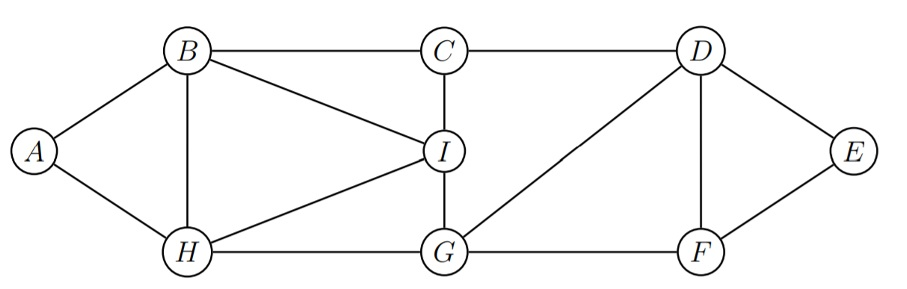
\includegraphics[scale=.74]{graph-image-v1.jpg}
\end{figure}

\begin{tabular}{|c|c|c|c|c|} \hline
  Vertex  &  \ha\  Color  \ha\ &   Discovery Time  & \ha\ Predecessor \ha\  & Finishing Time \\
  $u$ & $u.color$ & $u.d$ & $u.\pi$ & $ u.f$\\ \hline
  A & & & & \\ \hline
  B & & & &\\ \hline
  C & & & &\\ \hline
  D & & & &\\ \hline
  E & & & & \\ \hline
  F & & & &\\ \hline
  G & & & &\\ \hline
  H & & & &\\ \hline
  I & & & &\\ \hline
\end{tabular}

\vs\
\vs\


\pagebreak


\noindent{\bf Problem 4: }(15 points)

Consider the following graph.

\begin{figure}[!h]
\centering
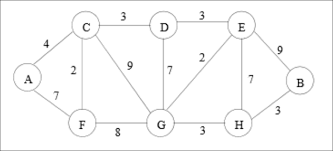
\includegraphics[scale=.74]{graph-prims-kruksal.png}
\end{figure}


\begin{itemize}
    \item[(a)]  Use Prim's algorithm to find a minimum-spanning-tree  for the above graph. Start from the vertex A. Draw the final MST and give the total weight.
    \item[(b)]  Use Kruksal's algorithm to find a minimum-spanning-tree  for the above graph.  Draw the final MST and give the total weight.
\end{itemize}

\noindent{\bf Problem 5: }(15 points)
\begin{itemize}
    \item[1)]  Let $G = (V,E,W)$ be a weighted connected (undirected) graph, where $V$ is the set of vertices, $E$ is the set of edges, $w_e \in W$ for each $e \in E$ is a nonnegative weight of the edge $e$. A spanning tree is defined as usual, namely $T = (V, T_E)$ where $T_E$ is a subset of  $E$ and $T$ is a tree. The width of a spanning tree $T$ is max $\{w_e | e \in T_E \}$.  Thus it is the most “expensive” edge in the tree. $T$ is a Minimum width spanning tree of $G$ if it is a spanning tree and achieves the minimum width among all spanning trees of $G.$ 
    \begin{itemize} 
        \item[(a)] Prove that any minimum spanning tree of $G$ is also a minimum width spanning tree of $G$. (Hint: You may use proof by contradiction.)
        \item[(b)] Show with an example that even if the weights of $G = (V,E,W)$ are all distinct, there could be more than one minimum width spanning tree.
    \end{itemize}
\end{itemize}

\vs\

\pagebreak

\vs\
\noindent{\bf Problem 6: }(15 points)
\vs\

\begin{itemize}
    \item[(a)] Draw a weighted graph that has exactly 5 different minimum spanning trees. Explain how you get the count.
    \item[(b)] Draw a weighted graph that has exactly 25 different minimum spanning trees. Explain how you get the count.
\end{itemize}


\vs\
\noindent{\bf Problem 10: }(15 points)
\vs\

Consider the collection of all undirected graphs with 10 nodes and 6 edges. Let M and m, respectively, be the
maximum and minimum number of connected components in any graph in the collection. If a graph has no selfloops
and there is at most one edge between any pair of nodes, which of the following is true? 
\begin{itemize}
    \item[(A)] M = 10, m = 10
    \item[(B)] M = 10, m = 1
    \item[(C)] M = 7, m = 4
    \item[(D)] M = 6, m = 4
    \item[(E)] M = 6, m = 3
\end{itemize}

Justify your selection by ruling out the other choices. Show two graphs that satisfy $M$ and $m$.

\end{document}
